\documentclass[UTF8,a4paper]{paper}
\usepackage{ctex}
\usepackage[utf8]{inputenc}
\usepackage{amsmath}
\usepackage{amssymb}
\usepackage{pdfpages}
\usepackage{graphicx}
\usepackage{xcolor}
\title{模式识别作业8}
\author{张蔚桐\ 2015011493\ 自55}
\begin {document}
\maketitle
\section{MDS算法的应用}
采用MDS算法对给出的数据二维化之后可以得到如图\ref{fig1}
所示的平面坐标图

\begin{figure}
\centering
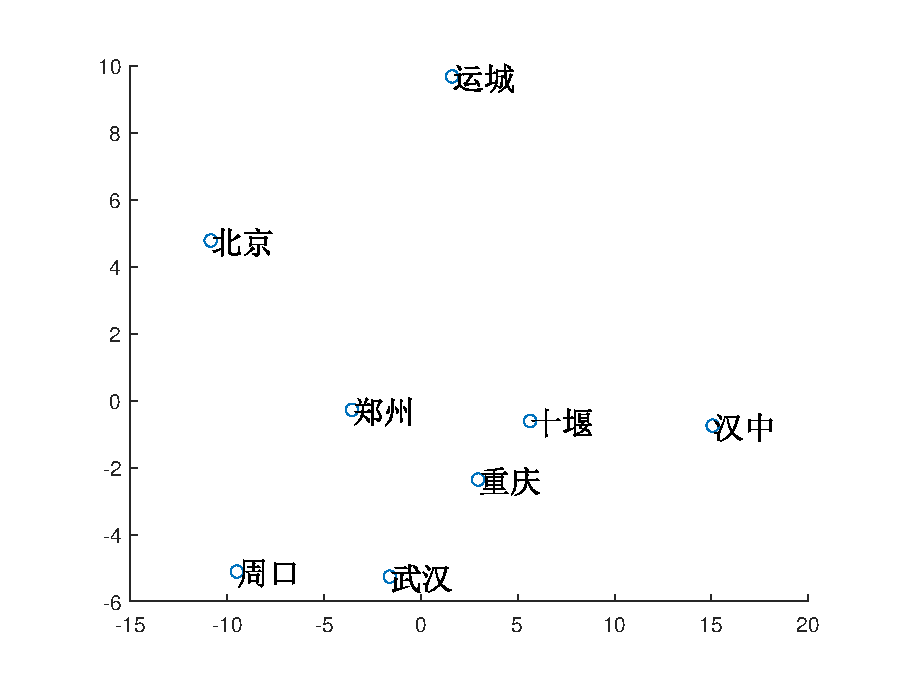
\includegraphics[width=\textwidth]{map.eps}
\caption{MDS方法处理过后的地图}
\label{fig1}
\end{figure}

对比图\ref{fig1}和实际情况我们可以看出,主要存在几点不同
\begin{enumerate}
\item 东西南北位置不对应

这一点使因为MDS算法没有相关的信息而出现的情况

\item 有些城市的相对地理位置不对

这一点可能是因为火车时间间隔和实际的地理情况有关,如西部地区
交通比较发达等

\end{enumerate}

\section{数据降维和处理}
我们使用PCA,LLE,TSNE三种方法对问题中给出的数据进行了降维
处理并使用相同的(40隐节点的单层神经网络)进行了测试,
测试正确率如图\ref{fig2}所示,可以看出测试正确率在
98\%以上

\begin{figure}
\centering
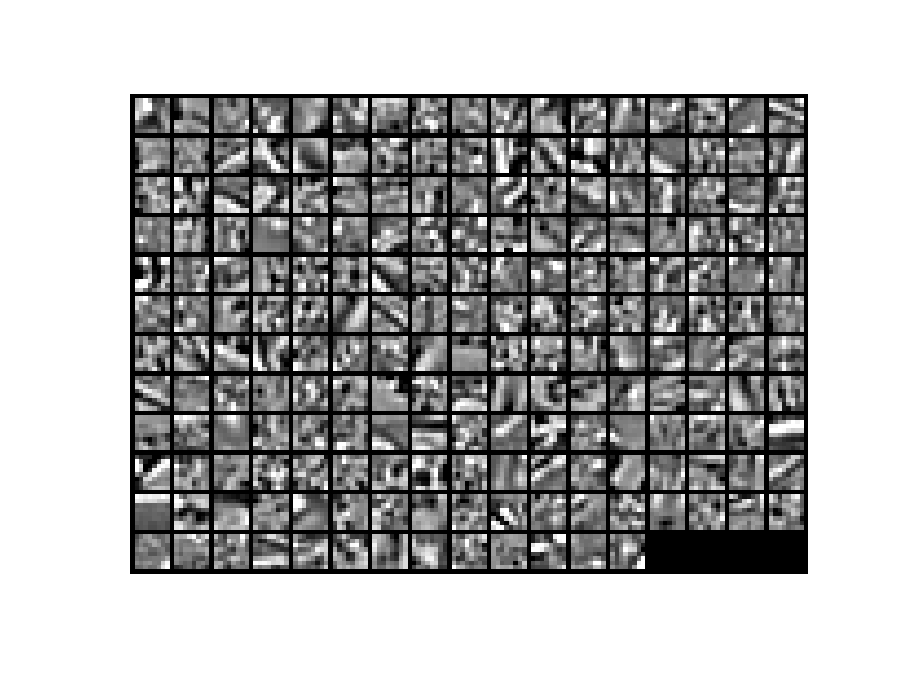
\includegraphics[width=\textwidth]{ori.eps}
\caption{不降维的测试混淆矩阵}
\label{fig2}
\end{figure}

\subsection{PCA}方法

PCA 方法的主要流程是将所给数据集进行类似KL变换,得到变换矩阵
和对应的方差分量。我们希望保证整个数据集的95\%左右的方差,
因此PCA采用了前133个变换向量,变换之后的二维展示效果和每个变
换对应的比例如图\ref{fig3}所示

\begin{figure}
\centering
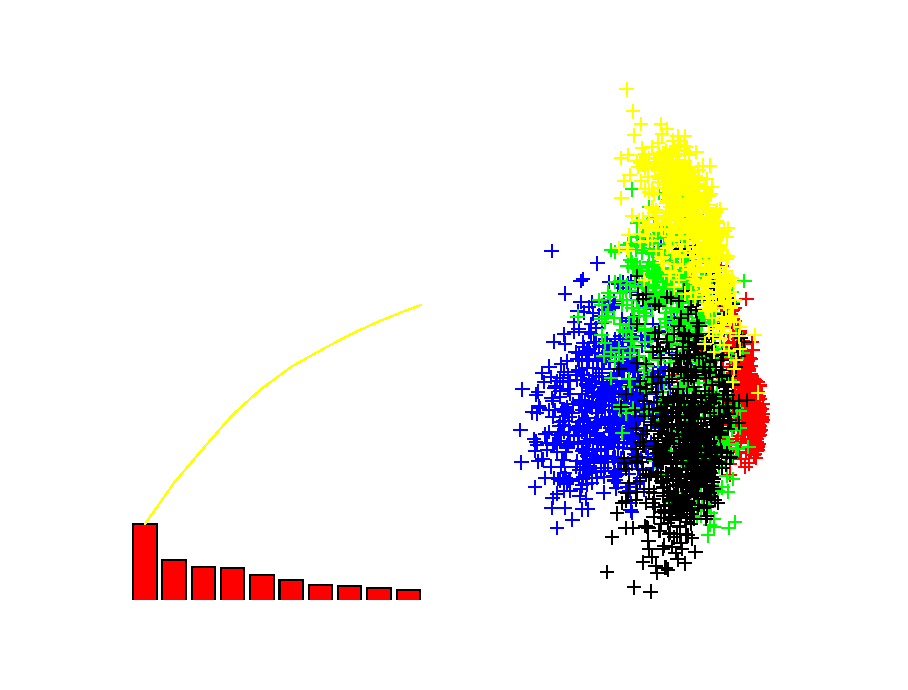
\includegraphics[width=\textwidth]{pca.eps}
\caption{PCA降维之后的二维平面显示}
\label{fig3}
\end{figure}

用和原始同样的神经网络对降维之后的数据加以训练,
得到的混淆矩阵如图\ref{fig4}所示,
可以看出虽然正确率有所下降
,但下降并不明显。但特征数是原来的$\frac{1}{6}$,
效果还是很满意的。

\begin{figure}
\centering
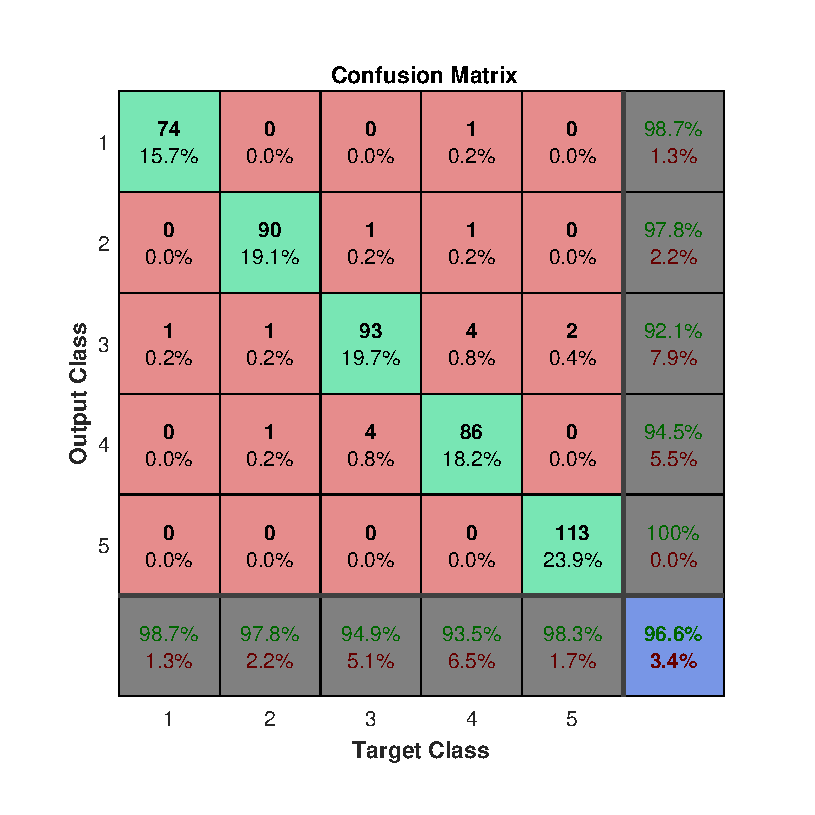
\includegraphics[width=\textwidth]{NNpca.eps}
\caption{PCA方法的测试正确率}
\label{fig4}
\end{figure}
\subsection{LLE方法}

LLE方法已经被完整的封装到给定的代码框架内,我们调用之后
直接输出前两维的情况即可得到需要的二维展示图,
如图\ref{fig5}所示

\begin{figure}
\centering
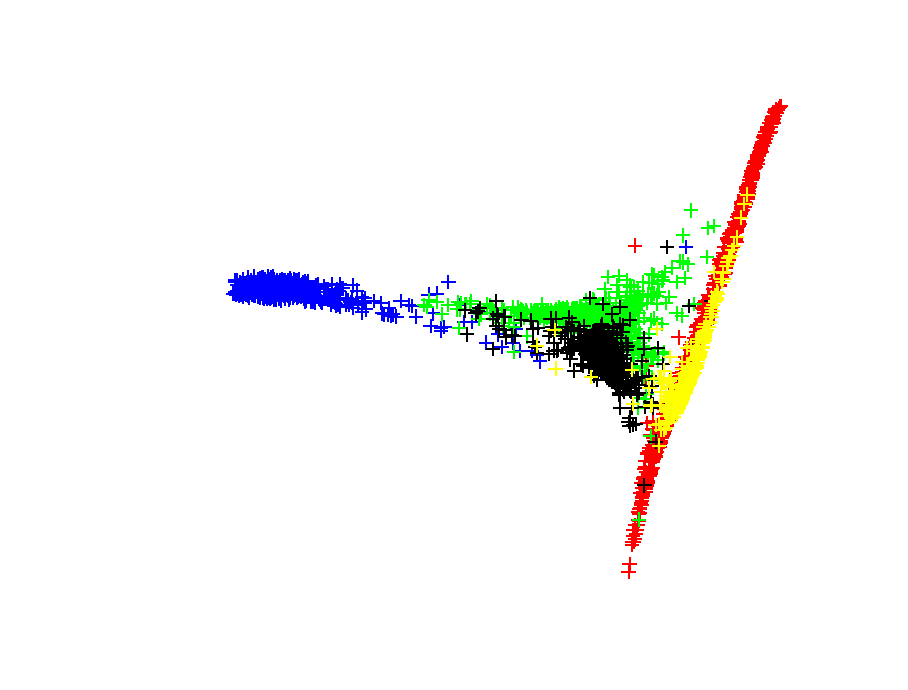
\includegraphics[width=\textwidth]{lle.eps}
\caption{LLE方法分类图}
\label{fig5}
\end{figure}

在试图对LLE方法压缩的数据进行训练的过程中我们发现,
LLE方法压缩的数据和数据本身有关,因此使用两组分别压缩的
测试集和训练集得到的训练——测试的效果很不好,我们对压缩之后
的训练集进行分割后测试训练集保留的测试部分正确率
如图\ref{fig6}
所示,可以看出,虽然仅剩下两维特征,
但是训练的效果还是比较好的。

\begin{figure}
\centering
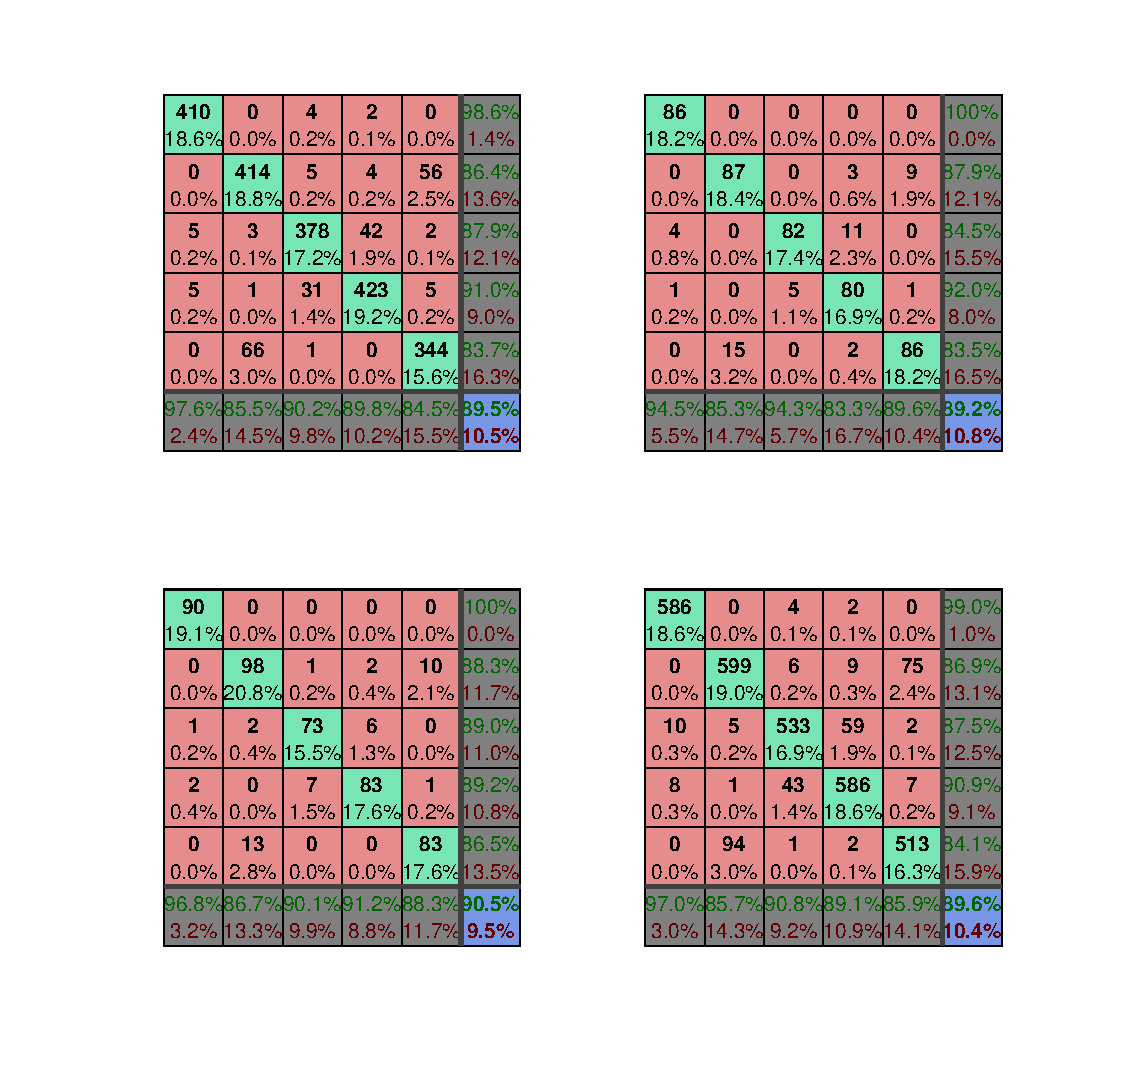
\includegraphics[width = \textwidth]{NNlle.eps}
\caption{LLE方法的测试正确率}
\label{fig6}
\end{figure}

\subsection{tSNE}方法
和LLE方法相同,tSNE方法也主要基于给定的算法框架。我们得到
二维平面显示如图\ref{fig7}所示

\begin{figure}
\centering
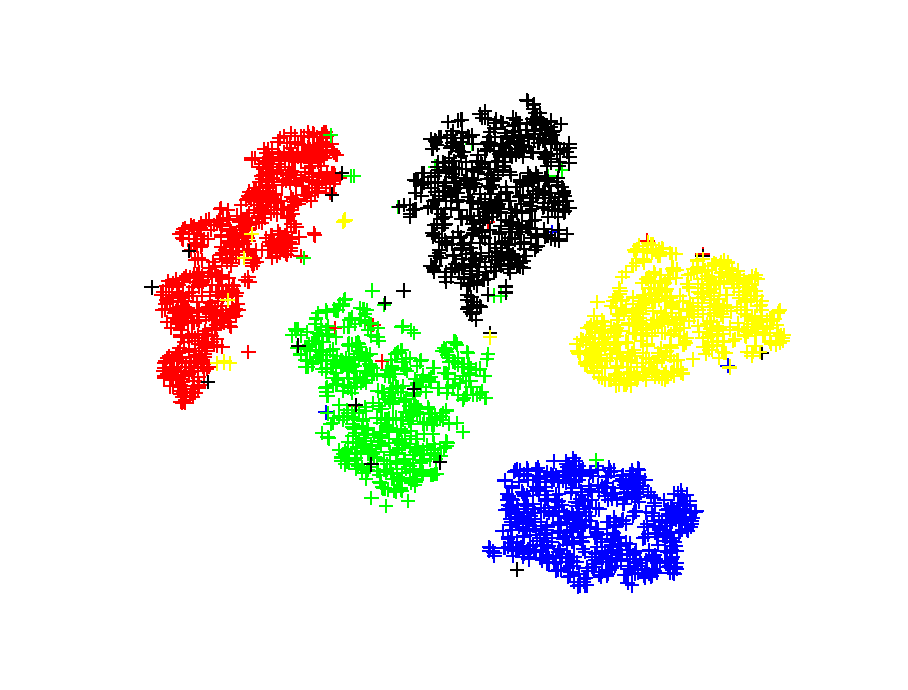
\includegraphics[width=\textwidth]{tsne.eps}
\caption{tSNE方法分类图}
\label{fig7}
\end{figure}

和LLE方法相同,这种方法的训练和数据集有关,因此我们需要在
训练集上分割出用于测试的部分,得到的训练效果如图\ref{fig8}
所示,效果还是比较理想的。

\begin{figure}
\centering
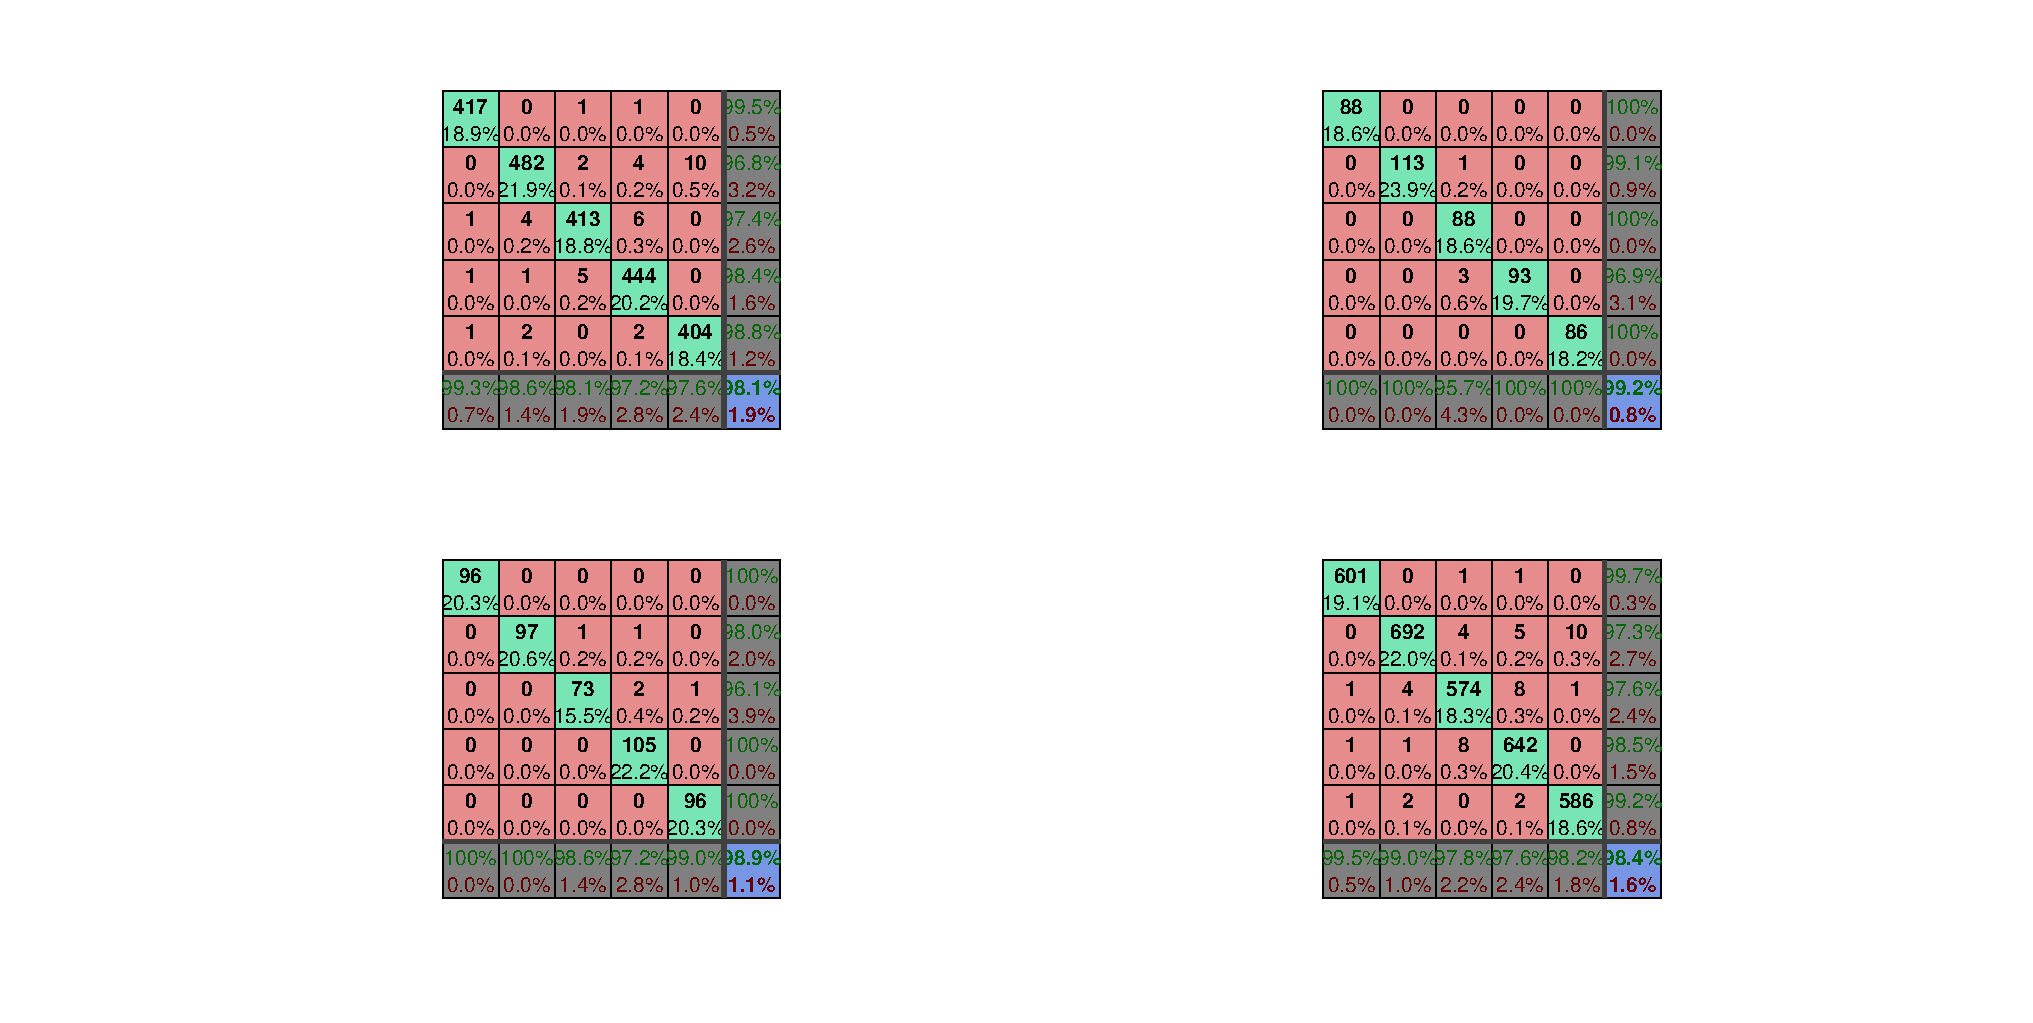
\includegraphics[width = \textwidth]{NNtsne.eps}
\caption{tSNE方法的测试正确率}
\label{fig8}
\end{figure}

总结三种降维方式,PCA线性降维,需要的计算量相对较小,后两种
可以处理非线性情况,其中就本题来看tSNE效果最好。

三种降维均对正确率有损失,但是降维程度较大,小部分的损失
是完全可以接受的。

\subsection{特征选取}
本题采用基于类内间隔和类间间隔的选择方法,为加快程序的运行效率,选取了50个特征并采用神经网络加以训练

首先程序将数据集分割为10份,之后每次选取9份进行训练,一份进行测试,训练集上采用$\mathrm{tr}S_b/\mathrm{tr}S_w$的指标进行特征选择并训练网络,十次分别测试得到的特征值。

特征选择过程中,我们认为每个特征之间是独立的,采用类内——类间准则为每个特征评分,选出最合适的前n个准则加以组合。

在这种条件下正确率在92\%,选取特征保存在index中,发现有很大的集中性,例如5,48,917号特征常常被选中,说明测试效果良好。

数据保存在ratio.mat 和index.mat中

注:按照要求已经将所有数据集剔除提交,如需重新运行代码需要自行添加数据集,代码运行时间可能较长





\end{document}